\section{Domänenmodellierung}

\begin{definition}{Domänenmodell}\\
Ein Domänenmodell ist ein vereinfachtes UML-Klassendiagramm zur Darstellung der Fachdomäne:
\begin{itemize}
    \item Konzepte als Klassen
    \item Eigenschaften als Attribute (ohne Typangabe)
    \item Beziehungen als Assoziationen mit Multiplizitäten
\end{itemize}
\includegraphics[width=\linewidth]{images/domänenmodell.png}
\end{definition}





\begin{KR}{Domänenmodell Erstellung}\\
\textbf{Schritt 1: Konzepte identifizieren}
\begin{itemize}
    \item Substantive aus Anforderungen extrahieren
    \item Kategorien prüfen:
    \begin{itemize}
        \item Physische Objekte (Produkte, Geräte)
        \item Kataloge und Listen
        \item Container (Warenkorb, Lager)
        \item Externe Systeme
        \item Rollen von Personen
        \item Artefakte (Pläne, Dokumente, Verträge)
        \item Zahlungsinstrumente (Transaktionen)
        \item \textbf{Wichtig:} Keine Softwareklassen modellieren!
    \end{itemize}
    \item Irrelevante Konzepte ausschließen
    \item Synonyme vereinheitlichen
\end{itemize}

\textbf{Schritt 2: Attribute definieren}
\begin{itemize}
    \item Nur wichtige/zentrale Attribute
    \item Typische Kategorien:
    \begin{itemize}
        \item Transaktionsdaten
        \item Teil-Ganzes Beziehungen
        \item Beschreibungen
        \item Verwendungszwecke
    \end{itemize}
    \item \textbf{Wichtig:} Beziehungen als Assoziationen, nicht als Attribute!
    \item Keine technischen IDs
    \item Keine abgeleiteten Werte
\end{itemize}

\textbf{Schritt 3: Beziehungen modellieren}
\begin{itemize}
    \item Assoziationen zwischen Konzepten identifizieren
    \item Multiplizitäten festlegen
    \item Art der Beziehung bestimmen
    \item Richtung der Assoziation falls nötig
    \item Rollen an Assoziationsenden benennen
\end{itemize}
\end{KR}


\begin{concept}{Domänenmodell Zweck}
\begin{itemize}
    \item Visualisierung der Fachdomäne für alle Stakeholder
    \item Grundlage für das spätere Softwaredesign
    \item Gemeinsames Verständnis der Begriffe und Zusammenhänge
    \item Dokumentation der fachlichen Strukturen
    \item Basis für die Kommunikation zwischen Entwicklung und Fachbereich
\end{itemize}
\end{concept}




\subsubsection{Analysemuster im Domänenmodell}

\begin{formula}{Analysemuster im Überblick} Details siehe nächste Seite\\
Bewährte Strukturen für wiederkehrende Modellierungssituationen:
\begin{itemize}
    \item \textbf{Beschreibungsklassen:} Trennung von Typ und Instanz
    \item \textbf{Generalisierung:} "ist-ein" Beziehungen
    \item \textbf{Komposition:} Starke Teil-Ganzes Beziehung
    \item \textbf{Zustände:} Eigene Zustandshierarchie
    \item \textbf{Rollen:} Verschiedene Funktionen eines Konzepts
    \item \textbf{Assoziationsklasse:} Attribute einer Beziehung
\end{itemize}
\end{formula}


\begin{KR}{Musterauswahl und Kombination}\\
Systematisches Vorgehen bei der Anwendung von Analysemustern:
\begin{enumerate}
    \item \textbf{Analyse der Situation}
    \begin{itemize}
        \item Konzepte und Beziehungen identifizieren, Attribute zuordnen
        \item Probleme im einfachen Modell erkennen (Bei Kombination)
    \end{itemize}

    \item \textbf{Passende Muster identifizieren}
    \begin{itemize}
        \item Beschreibungsklassen bei gleichartigen Objekten
        \item Generalisierung bei "ist-ein"-Beziehungen
        \item Komposition bei existenzabhängigen Teilen
        \item Zustände bei Objektlebenszyklen
        \item Rollen bei verschiedenen Funktionen
        \item Assoziationsklassen bei Beziehungsattributen
        \item Wertobjekte bei komplexen Werten
    \end{itemize}

    \item \textbf{Musterauswahl}
    \begin{itemize}
        \item Vor- und Nachteile abwägen 
        \item Komplexität vs. Nutzen bewerten
    \end{itemize}
    
    \item \textbf{Muster anwenden}
    \begin{itemize}
        \item Struktur des Musters übernehmen, an Kontext anpassen
        \item Konsistenz und fachliche Korrektheit sicherstellen
    \end{itemize}
    
    \item \textbf{Muster kombinieren}
    \begin{itemize}
        \item An Kontext anpassen und mit bestehenden Elementen verbinden
        \item Überschneidungen identifizieren und Konflikte auflösen
        \item Gesamtmodell harmonisieren
        \item Konsistenz und fachliche Korrektheit sicherstellen
    \end{itemize}
\end{enumerate}
\end{KR}


\begin{example2}{Prüfungsaufgabe: Konzeptidentifikation}\\
\textbf{Aufgabentext:} 
"Ein Bibliothekssystem verwaltet Bücher, die von Mitgliedern ausgeliehen werden können. Jedes Buch hat eine ISBN und mehrere Exemplare. Mitglieder können maximal 5 Bücher gleichzeitig für 4 Wochen ausleihen. Bei Überschreitung wird eine Mahngebühr fällig."
\vspace{2mm}\\
\textbf{Identifizierte Konzepte:}
Buch (Beschreibungsklasse), Exemplar (Physisches Objekt), Mitglied (Rolle), Ausleihe (Transaktion), Mahnung (Artefakt)
\vspace{2mm}\\
\textbf{Begründung:}
\begin{itemize}
    \item Buch/Exemplar: \\ Trennung wegen mehrfacher Exemplare (Beschreibungsmuster)
    \item Ausleihe: Verbindet Exemplar und Mitglied, hat Zeitbezug
    \item Mahnung: Entsteht bei Fristüberschreitung
\end{itemize}
\end{example2}

\columnbreak


\begin{concept}{Review eines Domänenmodells}
Checkliste für die Überprüfung:
\begin{itemize}
    \item \textbf{Fachliche Korrektheit}
    \begin{itemize}
        \item Alle relevanten Konzepte vorhanden?
        \item Begriffe aus der Fachdomäne verwendet?
        \item Beziehungen fachlich sinnvoll?
    \end{itemize}
    
    \item \textbf{Technische Korrektheit}
    \begin{itemize}
        \item UML-Notation korrekt?
        \item Multiplizitäten angegeben?
        \item Assoziationsnamen vorhanden?
    \end{itemize}
    
    \item \textbf{Modellqualität}
    \begin{itemize}
        \item Angemessener Detaillierungsgrad?
        \item Analysemuster sinnvoll eingesetzt?
        \item Keine Implementation vorweggenommen?
    \end{itemize}
\end{itemize}
\end{concept}

\begin{theorem}{Typische Modellierungsfehler vermeiden}
\begin{itemize}
    \item \textbf{Keine Softwareklassen modellieren}
    \begin{itemize}
        \item Manager-Klassen vermeiden
        \item Keine technischen Helper-Klassen
    \end{itemize}
    
    \item \textbf{Keine Operationen modellieren}
    \begin{itemize}
        \item Fokus auf Struktur, nicht Verhalten
        \item Keine CRUD-Operationen
    \end{itemize}
    
    \item \textbf{Richtige Abstraktionsebene wählen}
    \begin{itemize}
        \item Nicht zu detailliert oder abstrakt
        \item Fachliche Begriffe verwenden
    \end{itemize}
    
    \item \textbf{Assoziationen statt Attribute}
    \begin{itemize}
        \item Beziehungen als Assoziationen modellieren
        \item Keine Objekt-IDs als Attribute
    \end{itemize}
\end{itemize}
\end{theorem}

\begin{corollary}{Typische Modellierungsfehler}\\
\textbf{Fehler 1: Technische statt fachliche Klassen}
\begin{itemize}
    \item \textbf{Falsch:} CustomerManager, OrderController, DatabaseHandler
    \item \textbf{Richtig:} Kunde, Bestellung, Produkt
\end{itemize}

\textbf{Fehler 2: IDs als Attribute statt Assoziationen}
\begin{itemize}
    \item \textbf{Falsch:} customerId: String, orderId: Integer
    \item \textbf{Richtig:} Direkte Assoziation zwischen Kunde und Bestellung
\end{itemize}

\textbf{Fehler 3: Implementierungsdetails}
\begin{itemize}
    \item \textbf{Falsch:} saveToDatabase(), validateInput(), createPDF()
    \item \textbf{Richtig:} Keine Operationen im Domänenmodell
\end{itemize}
\end{corollary}

\begin{example2}{Typische Prüfungsaufgabe: Modell verbessern}\\
\textbf{Fehlerhaftes Modell:}
\begin{itemize}
    \item Klasse 'UserManager' mit CRUD-Operationen
    \item Attribute 'customerID' und 'orderID' statt Assoziationen
    \item Operation 'calculateTotal()' in Bestellung
    \item Technische Klasse "DatabaseConnection"
\end{itemize}

\textbf{Verbesserungen:}
\begin{itemize}
    \item 'UserManager' entfernen, stattdessen Beziehungen modellieren
    \item IDs durch direkte Assoziationen ersetzen
    \item Operationen entfernen (gehören ins Design)
    \item Technische Klassen entfernen
\end{itemize}
\end{example2}




\columnbreak

\subsubsection{Detaillierte Analysemuster}

\begin{concept}{1. Beschreibungsklassen}\\
Trennt die Beschreibung eines Typs von seinen konkreten Instanzen.

\textbf{Anwendung:}
\begin{itemize}
    \item Bei mehreren gleichartigen Objekten
    \item Gemeinsame unveränderliche Eigenschaften
    \item Vermeidung von Redundanz
\end{itemize}

\begin{minipage}{0.45\linewidth}
\textbf{Beispielstruktur:}
\begin{itemize}
    \item ProductDescription (Typ)
    \begin{itemize}
        \item price, description, itemID
    \end{itemize}
    \item Product (Instanz)
    \begin{itemize}
        \item serialNumber
    \end{itemize}
\end{itemize}
\end{minipage}
\begin{minipage}{0.5\linewidth}
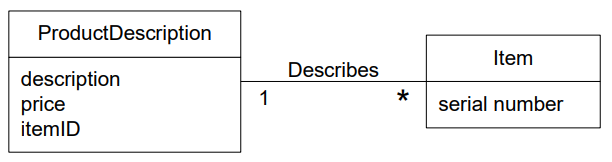
\includegraphics[width=\linewidth]{images/beschreibungsklasse_better.png}
\end{minipage}
\end{concept}

\begin{example2}{Beschreibungsklassen in der Praxis}
\textbf{Szenario:} Bibliothekssystem

\textbf{Problem:} 
Ein Buch kann mehrere physische Exemplare haben, die alle dieselben Grunddaten (Titel, Autor, ISBN) aber unterschiedliche Zustände (ausgeliehen, verfügbar) haben.

\textbf{Lösung:}
\begin{itemize}
    \item \textbf{Book} (Beschreibungsklasse)
    \begin{itemize}
        \item title, author, isbn, publisher
    \end{itemize}
    \item \textbf{BookCopy} (Instanzklasse)
    \begin{itemize}
        \item inventoryNumber, status, location
    \end{itemize}
    \item Assoziation: BookCopy "beschrieben durch" Book
\end{itemize}
\end{example2}

\begin{concept}{2. Generalisierung/Spezialisierung}\\
\textbf{Regeln:}
\begin{itemize}
    \item 100\% Regel: Jede Instanz der Spezialisierung ist auch Instanz der Generalisierung
    \item 'IS-A' Beziehung
    \item Gemeinsame Attribute/Assoziationen als Grund für Generalisierung
    \item Gemeinsame Eigenschaften in Basisklasse
    \item Spezifische Eigenschaften in Unterklassen
\end{itemize}

\textbf{Beispiele:}
\begin{itemize}
    \item Person → Student, Dozent
    \item Zahlung → Barzahlung, Kreditkartenzahlung
    \item Dokument → Rechnung, Lieferschein
\end{itemize}
\end{concept}

\begin{example2}{Generalisierung im Online-Shop}
\textbf{Szenario:} Versch. Zahlungsarten

\begin{minipage}[t]{0.58\linewidth}
\textbf{Struktur:}
\begin{itemize}
    \item \textbf{Payment} (abstrakt)
    \begin{itemize}
        \item amount, date, status
    \end{itemize}
    \item \textbf{CashPayment}
    \begin{itemize}
        \item receivedAmount, changeAmount
    \end{itemize}
    \item \textbf{CreditCardPayment}
    \begin{itemize}
        \item cardType, authorizationCode
    \end{itemize}
\end{itemize}
\end{minipage}
\begin{minipage}[t]{0.4\linewidth}
\textbf{Begründung:}
\begin{itemize}
    \item Gemeinsame Attribute \\in Payment
    \item Spezifische Attribute \\in Unterklassen
    \item Jede Zahlung ist\\ genau ein Typ
\end{itemize}
\end{minipage}

%add diagram showing payment hierarchy
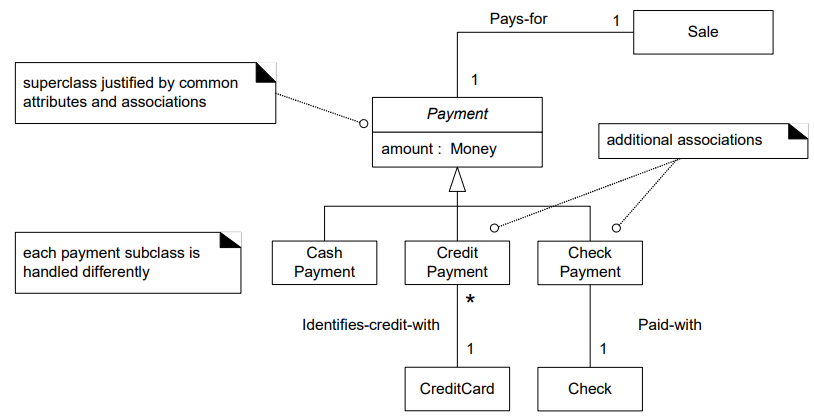
\includegraphics[width=\linewidth]{images/generalisierung_extended.png}
\end{example2}

\begin{concept}{3. Komposition}\\
Modelliert eine starke Teil-Ganzes Beziehung mit Existenzabhängigkeit der Teile.

\textbf{Eigenschaften:}
\begin{itemize}
    \item Teile können nicht ohne Ganzes existieren
    \item Teil gehört zu genau einem Ganzen
    \item Löschen des Ganzen löscht alle Teile
\end{itemize}

\textbf{Notation:}
\begin{itemize}
    \item Ausgefüllte Raute am "Ganzes"-Ende
    \item Multiplizität am "Teil"-Ende
\end{itemize}
\end{concept}

\begin{example2}{Komposition im Bestellsystem}\\
\textbf{Szenario:} Bestellung mit Bestellpositionen

\textbf{Struktur:}
\begin{itemize}
    \item \textbf{Order}
    \begin{itemize}
        \item orderDate, status
    \end{itemize}
    \item \textbf{OrderItem}
    \begin{itemize}
        \item quantity, price
    \end{itemize}
    \item Komposition von Order zu OrderItem (1 zu *)
\end{itemize}

\textbf{Begründung:}
\begin{itemize}
    \item OrderItems existieren nur im Kontext einer Order
    \item Löschen der Order löscht alle OrderItems
    \item Ein OrderItem gehört zu genau einer Order
\end{itemize}
\end{example2}

\begin{concept}{4. Zustandsmodellierung}\\
Modelliert Zustände als eigene Konzepthierarchie statt als Attribut.

\textbf{Vorteile:}
\begin{itemize}
    \item Klare Strukturierung der Zustände
    \item Vermeidet problematische Vererbung
    \item Erweiterbarkeit durch neue Zustandsklassen
    \item Vermeidung von if/else Kaskaden
    \item Zustandsspezifisches Verhalten möglich
\end{itemize}

\textbf{Beispielstruktur:}
\begin{itemize}
    \item OrderState (abstrakt)
    \begin{itemize}
        \item New, InProgress, Completed
    \end{itemize}
    \item Order "ist in" OrderState
\end{itemize}
%add image showing state pattern in domain model
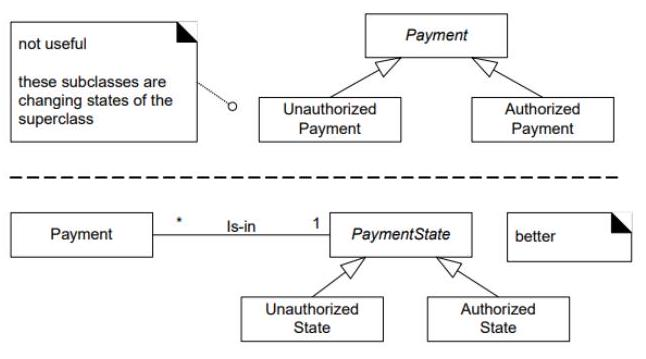
\includegraphics[width=0.9\linewidth]{images/2024_12_29_0d1d7b5551ea1b4b41bdg-07(1)}
\end{concept}


\begin{example2}{Zustandsmodellierung: Ticketsystem}\\
\textbf{Szenario:} Support-Tickets mit verschiedenen Status

\textbf{Falsche Modellierung:}
\begin{lstlisting}[language=Java, style=base]
class Ticket {
    enum Status {NEW, OPEN, IN_PROGRESS, RESOLVED, CLOSED}
    private Status status;
}
\end{lstlisting}

\textbf{Bessere Modellierung:}
\begin{itemize}
    \item \textbf{TicketState} (abstrakt)
    \begin{itemize}
        \item timestamp, changedBy
    \end{itemize}
    \item Konkrete Zustände:
    \begin{itemize}
        \item NewState: assignedTo
        \item OpenState: priority
        \item InProgressState: estimatedCompletion
        \item ResolvedState: solution
        \item ClosedState: closureReason
    \end{itemize}
\end{itemize}
\end{example2}

\begin{concept}{5. Rollen}\\
Modelliert verschiedene Funktionen eines Konzepts.

\textbf{Varianten:}
\begin{itemize}
    \item Rollen als eigene Konzepte
    \item Rollen als Assoziationsenden
    \item Rollen durch Generalisierung
\end{itemize}

\textbf{Anwendung:}
\begin{itemize}
    \item Bei verschiedenen Verantwortlichkeiten
    \item Wenn Rollen wechseln können
    \item Bei unterschiedlichen Beziehungen
\end{itemize}
\end{concept}


\begin{example2}{Rollenmuster: Universitätssystem}\\
\textbf{Szenario:} Person kann gleichzeitig Student und Tutor sein

\textbf{Variante 1: Rollen als Konzepte}
\begin{itemize}
    \item \textbf{Person}
    \begin{itemize}
        \item name, birthDate, address
    \end{itemize}
    \item \textbf{StudentRole}
    \begin{itemize}
        \item matriculationNumber, program
    \end{itemize}
    \item \textbf{TutorRole}
    \begin{itemize}
        \item department, hourlyRate
    \end{itemize}
\end{itemize}

\textbf{Variante 2: Generalisierung}
\begin{itemize}
    \item Person als Basisklasse
    \item Student und Tutor als Spezialisierungen
    \item Problem: Mehrfachrollen schwierig
\end{itemize}
%add diagram showing both variants
\end{example2}

\begin{concept}{6. Assoziationsklassen}\\
Modelliert Attribute einer Beziehung zwischen Konzepten, eigene Klasse für die Assoziation

\textbf{Einsatz wenn:}
\begin{itemize}
    \item Attribute zur Beziehung gehören
    \item Beziehung eigene Identität hat
    \item Mehrere Beziehungen möglich sind
\end{itemize}

\textbf{Notation:}
\begin{itemize}
    \item Gestrichelte Linie zur Assoziation
    \item Klasse enthält beziehungsspezifische Attribute
\end{itemize}
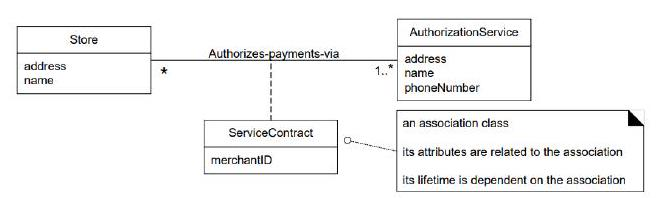
\includegraphics[width=\linewidth]{images/2024_12_29_0d1d7b5551ea1b4b41bdg-07}
\end{concept}


\begin{example2}{Assoziationsklasse: Kursbuchungssystem}\\
\textbf{Szenario:} Studenten können sich für Kurse einschreiben

\textbf{Struktur:}
\begin{itemize}
    \item \textbf{Student} und \textbf{Course} als Hauptkonzepte
    \item \textbf{Enrollment} als Assoziationsklasse:
    \begin{itemize}
        \item enrollmentDate
        \item grade
        \item attendance
        \item status
    \end{itemize}
\end{itemize}

\textbf{Begründung:}
\begin{itemize}
    \item Noten gehören zur Einschreibung
    \item Student kann mehrere Kurse belegen
    \item Kurs hat mehrere Studenten
    \item Einschreibungsdaten sind beziehungsspezifisch
\end{itemize}
%add diagram showing association class example
\end{example2}


\begin{concept}{7. Wertobjekte}
\begin{itemize}
    \item Masseinheiten als eigene Konzepte
    \item Zeitintervalle als Konzepte
    \item Vermeidet primitive Obsession
\end{itemize}
\end{concept}

\subsubsection{Mehr Info und Beispiele}


\begin{definition}{Optionale Elemente im Domänenmodell}
\begin{itemize}
    \item Optional: Aggregationen/Kompositionen
\end{itemize}
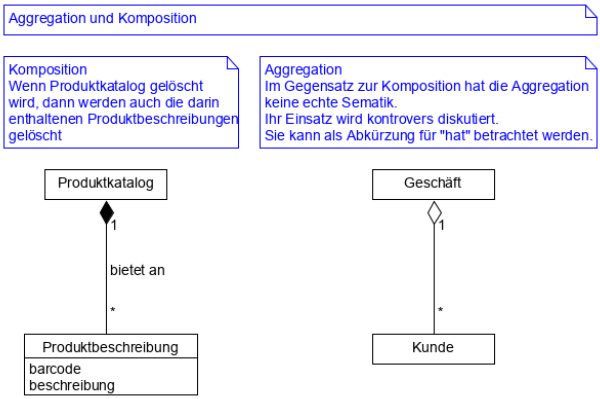
\includegraphics[width=\linewidth]{images/aggregation_komposition.png}
\begin{itemize}
    \item Optional: Generalisierung/Spezialisierung
\end{itemize}
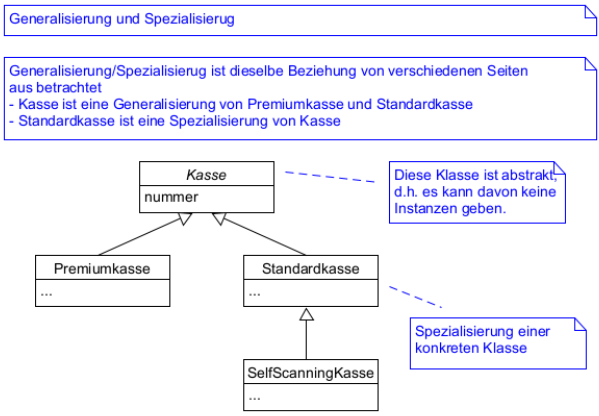
\includegraphics[width=\linewidth]{images/gener_spez.png}
\end{definition}

\columnbreak

\subsubsection{Vollständige Beispiele Domänenmodell}


\begin{example2}{Domänenmodell Online-Shop}\\
\textbf{Aufgabe:} Erstellen Sie ein Domänenmodell für einen Online-Shop mit Warenkorb-Funktion.

\textbf{Lösung:}
\begin{itemize}
    \item \textbf{Konzepte identifizieren:}
    \begin{itemize}
        \item Artikel (physisches Objekt)
        \item Artikelbeschreibung (Beschreibungsklasse)
        \item Warenkorb (Container)
        \item Bestellung (Transaktion)
        \item Kunde (Rolle)
    \end{itemize}
    \item \textbf{Attribute:}
    \begin{itemize}
        \item Artikelbeschreibung: name, preis, beschreibung
        \item Bestellung: datum, status
        \item Kunde: name, adresse
    \end{itemize}
    \item \textbf{Beziehungen:}
    \begin{itemize}
        \item Warenkorb gehört zu genau einem Kunde (Komposition)
        \item Warenkorb enthält beliebig viele Artikel
        \item Bestellung wird aus Warenkorb erstellt
    \end{itemize}
\end{itemize}
\end{example2}

\begin{example2}{Komplexes Domänenmodell: Reisebuchungssystem}\\
\textbf{Anforderung:} Modellieren Sie ein System für Pauschalreisen mit Flügen, Hotels und Aktivitäten.

\textbf{Verwendete Analysemuster:}
\begin{itemize}
    \item \textbf{Beschreibungsklassen:}
    \begin{itemize}
        \item Flugverbindung vs. konkreter Flug
        \item Hotelkategorie vs. konkretes Zimmer
        \item Aktivitätstyp vs. konkrete Durchführung
    \end{itemize}
    
    \item \textbf{Zustände:}
    \begin{itemize}
        \item Buchungszustände: angefragt, bestätigt, storniert
        \item Zahlungszustände: offen, teilbezahlt, vollständig
    \end{itemize}
    
    \item \textbf{Rollen:}
    \begin{itemize}
        \item Person als: Kunde, Reiseleiter, Kontaktperson
    \end{itemize}
    
    \item \textbf{Wertobjekte:}
    \begin{itemize}
        \item Geldbetrag mit Währung
        \item Zeitraum für Reisedauer
    \end{itemize}
\end{itemize}
%TODO: Beispieldiagramm
\end{example2}



